\documentclass[a4paper,norsk,11pt]{interaktiv}

% Importerte pakker
\usepackage{float}
\restylefloat{figure}
\usepackage{ifluatex}
\usepackage{subfigure}
\usepackage{tikz}
\usetikzlibrary{arrows}
\usepackage[parfill]{parskip}    		% Activate to begin paragraphs with an empty line rather than an indent
\usepackage{graphicx}

\ifluatex
  \usepackage{fontspec}
  \setmainfont{Calibri}
  \usepackage{unicode-math}
  \setmathfont{Cambria Math}
\else
  \usepackage[utf8]{inputenc}
\fi

\usepackage{url}

% Underfigurer
\renewcommand{\thesubfigure}{(\arabic{subfigure})}

% Overskrift
\emnekode{TMA4111}
\emnenavn{Matematikk 3 for MTELSYS}
\title{Integraltransformer}



% Nye kommandoer
\newcommand{\dee}{\mathop{}\!{d}}

\begin{document}
\pagenumbering{gobble}

\maketitle


Vi skal de neste tre ukene studere tre ting som ved første øyekast ser veldig vanskelige ut,
nemlig konvolusjon
\[
x(t)\ast y(t) = \int_{-\infty}^{\infty} x(\theta) y(t-\theta)\; d\theta,
\]
fouriertransform
\[
X(\omega) = \mathcal{F}\left\{ x(t) \right\}=\int_{-\infty}^{\infty} x(t)e^{-i\omega t}\;dt,
\]
og ensidig laplacetransform
\[
X(s)= \mathcal{L}\left\{ x(t) \right\}=\int_0^{\infty} x(t)e^{-st}\; dt.
\]
der $s=\sigma + i \omega$.
Disse tre dyrene her tar lang tid å forstå, 
men er på hver sin måte veldig viktige for analyse av alle slags lineære systemer, 
ikke bare elektriske.
Fouriertransform er et spesialtilfelle av laplacetransform (sett $\sigma=0$).
Konvolusjon er et slags merkelig produkt mellom funksjoner. 
En av de viktigste tingene å ta stilling til i starten,
er hva som kan puttes inn i disse dyrene. 

\begin{oppgave}{1}
Kan du fouriertransformere funksjonen $f(t)=1$?
\end{oppgave}

\begin{oppgave}{2}
Kan du laplacetransformere funksjonen $f(t)=1$?
\end{oppgave}

\begin{oppgave}{3}
Hva med $f(t)=e^{-|t|}$? (Prøv både laplace og fourier.)
\end{oppgave}

\begin{oppgave}{4}
Hva med $f(t)=\cos t$? (Prøv både laplace og fourier.)
\end{oppgave}


Vi var så vidt innom laplacetransform i første semester. 
Vi skal nå ta en liten repetisjon av hva det gikk i.
Vi brukte den til å løse ordinære differensiallikninger.

\begin{oppgave}{5}
Bruk laplacetransform til å løse initialverdiproblemet
\[
\ddot{x}(t)+x(t)=0 \quad x(0)=1.
\]
\end{oppgave}


Det er to spesielle funksjoner som er veldig viktige i elektroteknikken. 
Det ene er enhetssprangfunksjonen
\[
u(t)= \left\{ 
\begin{array}{ll}
0 & \mbox{ for } t<0\\
1 & \mbox{for } t\geq 0.
\end{array}
\right.
\]
som vi allerede kjenner til.
Man kan tenke på denne som en funksjon som slår noe på ved $t=0$. 
 \begin{center}
    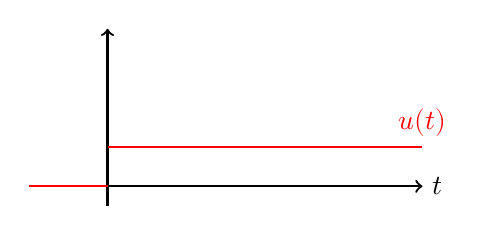
\begin{tikzpicture}[thick]
      \begin{scope}[xshift=5cm,yshift=-1cm]
          \draw[->] (-3.5,0) -- (1.5,0) node[right]{$t$};
          \draw[->] (-2.5,-0.25) -- (-2.5,2) ;
          \draw[-,red] (-3.5,0) -- (-2.5,0);
          \draw[-,red] (-2.5,0.5) -- (1.5,0.5) node[above]{$u(t)$};
      \end{scope}
    \end{tikzpicture}
  \end{center}


\begin{oppgave}{6}
Bruk laplacetransform til å løse initialverdiproblemet
\[
\ddot{x}(t)+x(t)=u(t-1) \quad x(0)=1.
\]
\end{oppgave}

Den andre har vi ikke sett ennå, 
og er ikke egentlig en funksjon. 
Den kalles Diracs deltafunksjon (\url{https://en.wikipedia.org/wiki/Dirac_delta_function}).
I starten kan man tenke på den som 
\[
\delta(t)= \left\{ 
\begin{array}{ll}
0 & \mbox{ for } t\neq 0\\
\infty & \mbox{for } t= 0.
\end{array}
\right.
\]

Her er en mer presis definisjon. La 
\begin{equation*}
g_k(t-a)=    
\begin{cases}
      1/k  & \text{for } a < t < a + k \\
      0 & \text{ellers} 
    \end{cases} 
\end{equation*}
Slik ser de ut:
 \begin{center}
    \begin{tikzpicture}[thick]
%      \draw[->] (-1.5,0) -- (1.5,0) node[right]{$x$};
%      \draw[->] (0,-1.5) -- (0,1.5) node[above]{$y$};
%      \filldraw[fill=blue!75!white,fill opacity=0.55] (-0.866,0.5)
%        [snake=coil,segment aspect=0,segment amplitude=1pt] --
%        (0.866,0.5) arc(30:-210:1cm);
%      \draw (0,0) circle (1cm);
%      \node[below right] at (1,0){$1$};
%      \node[below left] at (-1,0){$-1$};
%      \node[above left] at (0,1){$1$};
%      \node[below left] at (0,-1){$-1$};
%      \node[draw,fill=white,align=center] at (0,0){$75$ \%};

      \begin{scope}[xshift=5cm,yshift=-1cm]
          \draw[->] (-2.5,0) -- (1.5,0) node[right]{$x$};
          \draw[->] (-2.5,-0.25) -- (-2.5,2) node[above]{$y$};
          \draw[-,red] (-1,2) -- (-.875,2) node[right]{$g_{1/8}$};
          \draw[-,red] (-1,0.5) -- (-.5,0.5) node[right]{$g_{1/2}$};
          \draw[-,red] (-1,1) -- (-.75,1) node[right]{$g_{1/4}$};
%         \draw (2,0) arc(55:125:3.9cm) node[right,xshift=2cm,yshift=1.2cm]{$u(x,t)$};
%          \draw (0,0) -- (2*0.866,1);
%          \draw[snake=coil,segment aspect=0,segment amplitude=1pt]
%            (0,1) -- (2*0.866,1);
%          \draw (0,0.35) arc(90:30:0.35cm)
%            node[above,xshift=-0.05cm,yshift=0.05cm]{$\theta$};
%          \draw[snake=brace] (-0.05,0) --
%            node[left,xshift=-0.05cm]{$h$} (-0.05,1);
          \node[below] at (-1,0){$a$};
%          \node[left] at (0,2){$L$};
      \end{scope}
    \end{tikzpicture}
  \end{center}
Vi definerer
\begin{equation*}
\delta(t)=\lim_{k \to 0} g_k(t)=\begin{cases}
      \infty  & \text{for } t = a  \\
      0 & \text{ellers} 
    \end{cases} 
\end{equation*}
Deltafunksjonen brukes til å modellere impuls, 
altså energitilførsler der den påtrykte kraften er ekstremt høy
og ekstremt kortvarig, for eksempel hammerslag. 
Man kan også tenke på den som noe som plukker ut funksjonsverdier fra integraler:
\begin{equation*}
\int_0^{\infty} f(t)\delta(t-a)\; dt=\lim_{k \to 0}\frac{1}{k}\int_a^{a+k} f(t)\; dt=f(a).
\end{equation*}



Deltafunksjonen er strengt tatt ikke noe funksjon,
og heavisidefunksjonen er ikke deriverbar. 
Det kan allikevel være fruktbart å tenke på deltafunksjonen
som et forsøk på å sette opp den deriverte til heavisidefunksjonen.
Deltafunksjonen er et veldig viktig verktøy for alle signalbehandlere, 
for den representerer et signal som inneholder like mye av alle frekvenskomponenter. 
Det sies at Lars Ottar Svaasand tok med seg pistol og fyrte av et skudd inne i Nidarosdomen i forbindelse med et oppdrag der han skulle analysere akustikken i rommet. 
Paul Dirac, som oppfant deltafunksjonalen, fikk nobelprisen i 1933 med Erwin Schrödinger for sitt arbeid med kvantemekanikk \url{https://en.wikipedia.org/wiki/Paul_Dirac}.


\begin{oppgave}{7}
Finn laplacetransformen til deltafunksjonalen.
\end{oppgave}


\begin{oppgave}{8}
Bruk laplacetransform til å løse initialverdiproblemet
\[
\ddot{x}(t)+x(t)=\delta(t-1) \quad x(0)=1.
\]
\end{oppgave}

\end{document}
